\documentclass[suppldata]{interact}
%\documentclass{article}


\usepackage[caption=false]{subfig} 
\usepackage{subcaption}
\usepackage{graphicx}
\usepackage{booktabs}
\usepackage{caption}
\usepackage{lscape}
\usepackage{rotating}
\usepackage{longtable}
\usepackage{enumitem}
\usepackage{amsmath}
\usepackage{array}
\usepackage{multirow}

\begin{document}


\title{  Surface Roughness Prediction of EN8 components using deep learning neural network}
\author{
\name{Ghanshyam Patel\textsuperscript{a}\thanks{CONTACT : Ghanshyam Patel Email: Ghanshyam.pphd22@sot.pdpu.ac.in} and M.B.Kiran\textsuperscript{a}}
\affil{\textsuperscript{a}Department of Mechanical Engineering,School of Technology,Pandit Deendayal Energy University}
}
\maketitle

\begin{abstract}
 EN8  is widely used in die making industry. The surface roughness of the die, while machining on EDM (Electric Discharge Machining) depends upon the process parameters of the machine \cite{joshi2020edm}. The evaluation of surface roughness has gained a lot of significance because of its ability to assess the functionality of a component. Knowing surface roughness makes it possible to predict whether a component will succeed or fail when put into service. This has motivated several researchers to work on predicting or measuring surface roughness in the past.   To predict surface roughness in electrical discharge machining (EDM) of EN8 steel, an artificial neural network (ANN) model is developed. Machining parameters including pulse on time($T_{on}$), pulse off time($T_{off}$) and peak current($I_p$),  are considered as input neurons, and the main types of surface roughness parameters, $R_a$, $R_q$, $R_z$, $R_p$, $R_v$, are used as output neurons.   Experiments are conducted based on Response surface method (RSM). Feedforward neural network models are developed using input layer with 3 neurons ,one hidden layer containing varying neurons, from 3 to 10. Results obtained from two prediction models  of RSM and ANN are compared. It was found that ANN model give best results. Four different training algorithms- are compared to select the best are the Levenberg-Marquardt(LM), Gradien Descent (GD), Gradient Descent Ascent(GDA), Root Mean Square Prop (RP). The best network is selected based on minimum mean squared error (MSE), minimum Mean Absolute Percentage Error (MAPE) and the highest coefficient determination ($R^2$). Network trained with LM algorithm is found to be the best ANN model to predict surface roughness parameters such as, Ra,Rq and Rv and GD algorithim is best for Rz and Rp. Using separate testing set, the network is also tested and it is observed that the experimental and predicted values are in proximity to each other.
  \end{abstract}
 \begin{keywords}
     Roughness measurement, Response surface method (RSM), Electrical discharge machining (EDM),Roughness prediction, Artificial neural network (ANN)
\end{keywords}

\section{Introduction}
Surface roughness is a significant parameter of any machined component. By knowing the surface roughness, it is possible to determine the suitability of the component when it is put into service. Thus, it can be considered an index of the quality of the product.  Many aerospace components such as engine piston heads, landing gear etc., are being manufactured by EDM. It is popular because the desired surface finish can be achieved easily, even with hard-to-machine materials. In this machining process, copper or any conductive metal electrode is used as the negative terminal, and the component to be machined is connected to the positive terminal. A very high temperature generates enough spark for enough heat to erode the workpiece component. The dielectric liquid will constantly flush out tiny particles from the machined surface to cool metal pieces and electrodes. It also controls the temperature so that the surface is not damaged. 
Surface roughness is a vital parameter in all industrial applications including Die making. Since Artificial intelligence's(AI) invention, many researchers have been applying it to many fields, including die making.A popular method for extracting information from unstructured data is the artificial neural network. The extensive connectivity of neurons used in model-based ANN design enhances performance.  The input, hidden, and output layers are used by the algorithm presented in this paper. This algorithm determines an initial set of weights and specifies how weights will be applied to improve performance during the training phase. A neuron's reaction to a signal it receives is controlled by an activation function. The sigmoid function is the most frequently utilized. The objective of the current research work is to develop an AI based model to predict surface roughness parameters-$R_a$, $R_q$, $R_z$, $R_p$, $R_v$. Earlier attempts by researchers included only prediction of $R_a$ as roughness parameter. Complete characterization of dies require $R_q$, $R_z$, $R_p$, $R_v$ parameters (Table\ref{tab:rapp}) as well. In this context the current research work assumes special significance.
\begin{table} [hbtp] 
    \centering
    \caption{Types of Surface Roughness Parameters and its Industrial Applications}
    \label{tab:rapp}
    \begin{tabular}{|c|l|p{0.6\linewidth}| }  \hline
        \textbf{Roughness} & \textbf{Full Name} & \textbf{Industrial Applications} \\ \hline
        Ra & Arithmetic Average Roughness & Quality control in manufacturing, functional performance of components, aesthetics in consumer products. \\ \hline
        Rq & Root Mean Square Roughness & Tribology studies, friction and wear resistance optimization, surface coating applications. \\ \hline
        Rz & Maximum Height of the Profile & Functional performance in sealing surfaces, tribology studies, adhesion in surface coatings. \\ \hline
        Rp & Maximum Peak Height & Friction and wear resistance optimization, adhesive bonding in assembly processes. \\ \hline
        Rv & Maximum Valley Depth & Friction and wear resistance optimization, adhesive bonding in assembly processes. \\ \hline
       
    \end{tabular}
\end{table}
\clearpage 
  \section{Literature survey}  

  \begin{longtable}  
 {|p{1.1cm}|p{1.6cm}|p{1.3cm}|p{2cm}|p{1.8cm}|p{1cm}|p{2.5cm}|p{2cm}|}
 \caption{ A Literature survey}\\
\hline

\textbf{Year} & \textbf{Author } & \textbf{Process } & \textbf{Material} & \textbf{Input parameter} &   \textbf{Objec-tive} & \textbf{Technique} & \textbf{Remark} \\ \hline 
 \endfirsthead

  \multicolumn{8}{c}%
  {{\bfseries \tablename\ \thetable{} -- continued from previous page}} \\
  \hline
  \textbf{Year} & \textbf{Author } & \textbf{Process } & \textbf{Material} & \textbf{Input parameter} &   \textbf{Objec-tive} & \textbf{Technique} & \textbf{Remark} \\
  \hline
  \endhead
   \multicolumn{8}{r}{{Continued on next page}} \\ 
  \endfoot
  \endlastfoot

   \cite{joshi2020edm}2020&Anurag Joshi  &EDM&EN8&Ton, Toff, wire feed&Ra&ERR and MRR & Low MRR \\  \hline
   \cite{ahmad2016optimization}2016&M.M. Ahmad & EDM &Titanium grade-2&Ton, Toff, Ip&Ra& Regression&MRR\\ \hline 
   \cite{aich2014modeling}2013&Ushasta Aich&EDM&HSS & Ton. Toff,Ip,& MRR & SVM, PSO,FFD & Optimization \\ \hline  

   \cite{balasubramaniyan2021wire}2021& Balsubra maniyan &WEDM & Nitinol  SMA Alloy &Ton,Toff,Ip, Vs, Ac  &Ra&MRR,RSM-CCD&Optimum Condition for MRR,Ra  \\ \hline
    \cite{das2014prediction}2015&Milan Kumar& EDM &EN31& Ip,Vp, Ton, Toff & Ra & LM,SCX,GDX & ANN=99\% RSM=98\% \\  \hline 
    \cite{giusti2020image}2020 &Alessandro Giusti& EDM &W300 ASP23 ,STAVAX & Steel& Ra &CNN-LeNet MODEL&Ra Prediction \\ \hline
	\cite{goyal2021optimization}2021&Ashish Goyal &EDM&Titanium luminide& Ton,Toff, Ip,&Ra & ANOVA & Ra decrease with Toff, increase with Ton,Ip \\ \hline
	\cite{naresh2020artificial}2020&Naresh &WEDM&NITINOL&Ton, Toff,Vp &Ra	&Adaptive neuro-fuzzy(ANFIS),LM	&MRR, Ra \\ \hline 
	\cite{park2016machine}2016&Je-Kang Park&N/a&Stone,Wood, Silicon wafer&  Surface&Defect detect&CNN, PSO&CNN netter than PSO\\ \hline 
	\cite{patel2009determination}2009&K.M.Patel&EDM&f Al2O3/SiC&Ton,Ip, Vg, Duty cycle&Ra&RSM,ANOVA & Ton is dominant for Ra \\ \hline
	\cite{patel2019texture}2019&Dhiren Patel& Milling &Al& Machined&Ra&GLCM,J48, RF,RBF, SVM, GLCM,& RF,ANN 99 \% accuracy \\ \hline
	\cite{paturi2021machine}2012 & Uma,Paturi & WEDM &Inconel 718 & Ip,Ton&Ra & ANN SVM RSM& SVM Better than ANN,RSM GA Opt \\ \hline
	\cite{paul2019multi}2019&R.R.Paul&EDM&Inconel 800&Ton,Toff,Ip&Ra&Multi objective optimization \& ratio analysis&Optimization of 
              parameters\\ \hline 
	\cite{routara2020investigation}2020&B.C.Routara& EDM &T6-Al7075 &Toff,Ip,Spark Gap &MRR, WTR, Ra &TOPSIS & MRR higher in Rotary mode\\ 
                 \hline 
	\cite{saeedi2021measurement}2020&Jamal Saeedi,&EDM&Steel&EDM machining  &Ra &CNN,VGG, AlexNet, ResNet & CNN based regression and classifier\\ \hline
	\cite{shivanna2014evaluation}2014&Shivanna&EDM& Steel&Ton,Ip&Sa,Sq, etc. &MATLAB&CCD,Confocal microscope\\ \hline 
%	\cite{srikanth2021optimization}2020& srikanth&EDM &Ti-6Al-4V &Ton,Toff,Ip, &MRR, TWR&MOORA& Optimization\\ \hline
	\cite{singh2022machine}2022& Ranjit Sigh&EDM&Cu-SMA&Ip,Ton,TWR&Ra&GA,TELBO&ANOVA Optimization \\ \hline
	\cite{ulas2020surface}2020 & Mustafa Ulas& WEDM & Al7075 Aluminum alloy & Vp,Ton,WFR &Ra& WDM,SVR & W-ELM results are good\\ \hline
	\cite{vakharia2022experimental}2022&Vinay Vakhria&WEDM&NITINOL&Ton,Toff,Ip&Ra&SinGAN, KNN, Alexnet ,DenseNet&SinGAN is effective\\ 
             \hline
	\cite{varol2021estimating}2021&Hatice Varol ,&EDM&Inconel 718&Ton, Toff, Ip& Ra&ANN, GEP, ANN& better than GEP\\ \hline 
	\cite{yogesh2021predicton}2020&Yogesh&WEDM&Aluminum composites&Ton, Toff, Ip& Ra, MRR&Decision tree, Nieve Byes& MRR \\ \hline
 \cite{zhang2023prediction}2023&Zhang&SLM&316L Stainless steel&Laser power, scanning speed and pitch& Ra &BPNN& No relation between Ra and Rel.Density \\ \hline
 \cite{kundrak2021accuracy}2021&Kundark&Turning, Grinding&Steel&Feed, DOC, Speed& 2D,3D analysis& Rs, Rq, Rz, Rsk, Rku & Accuracy and Topography  \\ \hline
 
\end{longtable}
\begin{minipage}{0.9\textwidth}
  \centering
    \captionof{table}{ Abreviations}
      \begin{tabular}{|p{0.4\linewidth}|p{0.4\linewidth}|p{0.4\linewidth}|}
      \hline
       EDM: Electric Discharge machine   & Ton : Pulse time on & Toff: Pulse time off \\  \hline 
  Ip:Pulsating current &  WEDM: Wire Electric Discharge Machining & Ra :Average surface Roughness \\ \hline
  Vp : Peak Voltage & MRR: Material removal rate &  SVR : Support vector Regression \\ \hline
  ANN : Automatic Neural network &  TWR: Tool Wear rate & RSM:Response surface Method\\  \hline
  ANOVA : Analysis of variance & CCD: Charged couple camera & ~\\ \hline
    \end{tabular}
   \label{tab:abr_label}
 \end{minipage}
 %\end{table}
 \clearpage
  Anurag et al. focus on the EN8 material utilized on the EDM machine in this study performs better than typical mild steel, which has carbon levels between 0.3 and 0.6\%. For higher values of the process parameters, the MRR is proportional to the EWR Electrode wear rate  
\textbf{\cite{joshi2020edm}}.

 Mustafaiz et al. investigate L18 Orthogonal Array (OA) tests were conducted using input factors such as Peak Current, Duty Cycle, and Voltage Gap. Studies were conducted to determine how machining parameters impacted responses like MRR \textbf{\cite{ahmad2016optimization}}.

 Ushasta Aich et al In this study, support vector machines, and PSO are employed to create EDM modeling frameworks. Models for MRR and Ra are created using SVM. To confirm the models' correctness and applicability, testing data sets are used to evaluate them \textbf{\cite{aich2014modeling}}.

 Balsubramaniam et al.focus the major focus of this study is wire electric discharge machining (W-EDM), which is used in SMA. When analyzing machining parameters, such as surface and material removal, current, servo voltage, and pulse on time were taken into account. pulse-free time. Parametric analysis was completed after the response surface approach-based central composite design \textbf{\cite{balasubramaniyan2021wire}}. 

The author investigate an ANN model has been created by the authors to forecast the surface roughness of EN 31 steel. Average roughness (Ra) is the output neuron, whereas machining parameters are the input neurons. A CCD serves to conduct experiments. Based on performance indicators, the best network is chosen after comparing several training techniques. Results from the L-M algorithm are good. When predicting surface roughness, the ANN model outperforms the RSM model. To examine how process variables affect results, 3D surface plots are employed \textbf{\cite{das2014prediction}}. 

 Allesandro Giusti et al. investigate a Convolutional Neural Network is employed in a cheap optical measurement system that is combined with an EDM machine to forecast Ra values. Experimental results show that predictions made at different roughness levels are accurate. This is an effective method for characterizing and controlling the roughness of surfaces in machining operations \textbf{\cite{giusti2020image}}.

Ashish Goyal et al. use surface roughness optimization on an EDM machine. The Taguchi approach has optimized the results that were achieved. ANOVA analysis reveals important criteria for enhancing surface roughness\textbf{\cite{goyal2021optimization}}.

 Naresh et al focus on Levenberg-Marquardt (LM) algorithms. It was discovered that LM with 10 neurons was the ideal algorithm and number of neurons in the hidden layer for ANN models \textbf{\cite{naresh2020artificial}}.

 Je-Kang Park et al.focus on artificial intelligence (AI) and smart sensors to automatically detect surface flaws in components. The suggested technique uses CNN-based image processing to find wear, scratches, and burrs. The efficiency of a single CNN network for assessing various sorts of flaws on textured and non-textured surfaces was demonstrated through the construction and testing of several neural networks \textbf{\cite{park2016machine}}.

 R.K.Patel et al;,focus on  Sorface roughness and EDM machining parameters Ton, Vgap, Duty cycle. Using Response surface Method  Ton is found o be dominant parameters\textbf{\cite{patel2009determination}} .

 Dhiren Patel et al. focus on  machine learning and image processing techniques are used to identify surface quality from machining surfaces. It offers a technique that uses machine learning algorithms to characterize collected photos by extracting statistical information from them. Results with the ANN and RF algorithms demonstrate remarkable accuracy. This study provides a practical method for evaluating machined surfaces' quality, which is advantageous to sectors including manufacturing and quality control \textbf{\cite{patel2019texture}}.

 Uma Maheswari,Reddy Patauri et al. Surface roughness significantly improves by 61.31 when the GA technique is used. These outcomes represent quick and precise WEDM of Inconel 718 prediction and optimization approaches \textbf{\cite{paturi2021machine}}.

 T. R. Paul et al. investigate the optimization process parameters in Inconel 800 EDM using a hybrid approach. It is very simple to use MOORA, or multi-objective optimization on the basis of ratio analysis, and it is also very simple mathematically.\textbf{\cite{paul2019multi}}.

 Routara et al. focus on the EDM machining properties of T6-Al7075. For both rotary and steady tool modes, the parameters Tonne, Toff, Ip, and voltage are used. MRR TWR, Ra, and Rq optimization for responses has been examined \textbf{\cite{routara2020investigation}}.

Jamal Seedi et al. investigate the research describes the use of deep neural networks in an industrial measurement system for determining surface roughness and fault detection on degraded steelwork parts. The suggested techniques are superior to others.  By combining CNN-based regression with CNN-based classification, we achieve accurate roughness estimation (7.32\% error), high defect detection accuracy (97.26\%), and precise localization (99.09\% area under the ROC curve)\textbf{\cite{saeedi2021measurement}}.  

 Shivanna et al use this study compares 3D surface roughness metrics using a confocal and CCD camera using aluminum as a specimen metal. The vision approach is a revolutionary technique.
\textbf{\cite{shivanna2014evaluation}}.
 Ranjit Singh et al In this study, EDM settings for a Cu-based shape memory alloy are optimized using machine learning techniques. The study examines how dimensional deviation and tool wear rate are affected by process parameters. The study makes use of a central composite design matrix and employs 2-D and 3-D graphs to illustrate response parameter behavior. Cu-based SMA machining in EDM processes and optimization by Genetic Algorithm, and Teacher Learning-based optimization approaches both involve machine learning \textbf{\cite{singh2022machine}}.

 Mustafa Ulas et al.focus on Aluminum alloys are precisely machined using WEDM and can estimate surface roughness, saving time and money compared to experimentation. Al7075 aluminum alloy experiments were conducted with various WEDM parameters, and machine-learning models for surface roughness prediction were built. The model has the accuracy of 0.9720 and has the most potential for use in manufacturing WEDM-produced parts \textbf{\cite{ulas2020surface}} .

 Vinay Vakharia et al. focus on Nitinol in manufacturing for biomedical and aeronautical applications is examined in this research. The difficulty of producing desired surface characteristics in machined components is discussed in the paper. FESEM (Electro Microscope) is utilized to analyze the surfaces of Nitinol specimens after wiring electrical discharge machining. Surface morphology and its link to process parameters are predicted using deep learning models, such as SinGAN and DenseNet. A useful tool for surface image prediction in manufacturing, the DenseNet model has great accuracy \textbf{\cite{vakharia2022experimental}}.

 Hatice Varol et al use the metal alloy Inconel 718 have excellent mechanical, corrosion-resistance, and high-temperature performance characteristics. However, problems arise from their low machinability and the necessity for expensive tools in conventional machining techniques. For cutting hard materials, non-traditional production techniques like electrical discharge machining offer an affordable solution. An artificial intelligence model for evaluating surface roughness based on process parameters was developed using ANN and GEP\textbf{\cite{varol2021estimating}}.
 Yogesh et al. draw attention to the difficulties in determining the ideal parameters for the highest MRR and the lowest Ra as well as the limitations of conventional testing techniques. The suggested approach uses Decision Tree and Naive Bayes algorithms to forecast SR and MRR, saving time and important resources. The emphasis is especially on the EDM machining of aluminum composites, demonstrating how the algorithms can be used in this situation\textbf{\cite{yogesh2021predicton}}.

 Zhang et al. focus on .selective laser melting (SLM) used back propagation neural networks (BPNN)which quickly predict the surface roughness with high prediction accuracy \textbf{\cite{zhang2023prediction}}.

 Kundrak et al. focus on surface roughness of machined hard material with Ra,Rq,Rz,Rsk,Rku parameter textbf{\cite{kundrak2021accuracy}}.
\section{Methodology}
The steps mentioned below are used while performing research.
\begin{enumerate}
             \item Specimen preparation.
	      \item Surface roughness measurement .
            \item Development of model using Artificial Neural Network (ANN).
            \item Prediction using RSM. 
            \item Prediction using ANN. 
\end{enumerate}
\subsection{Specimen preparation}
 
 Generally, for three parameters and at three levels need 27 ($4^3$) numbers of experiments to be conducted.  Central composite design of experiment suggests very less number of experiments to predict optimized conditions among the assigned parameters with their levels.  Taguchi L27 array is found to be suitable for this experimental approach of study. Hence, only 27 experiments are required to be conducted to find the combination of levels of parameters, which give the optimal result. Analysis of Variance (ANOVA) is performed to observe the effects of process parameters.	By altering settings during an EDM machining operation, specimens are prepared. In Table \ref{tab:input}, $I_p$, $T_{on}$, $T_{off}$ are variables and peak Voltage is kept constant When performing an EDM operation on specimens, die electric fluid is employed.
  \begin{figure}[htbp]
          \begin{minipage}{0.5\textwidth}
        \centering
        \includegraphics[width= 0.5\linewidth]{MMP-27 No -EDM-speciemans.jpg}
        \caption{EDM 27 Nos.specimens on EN8 plate}
        \label{fig:speciman}
      \end{minipage} 
    \begin{minipage}{0.4\textwidth}
        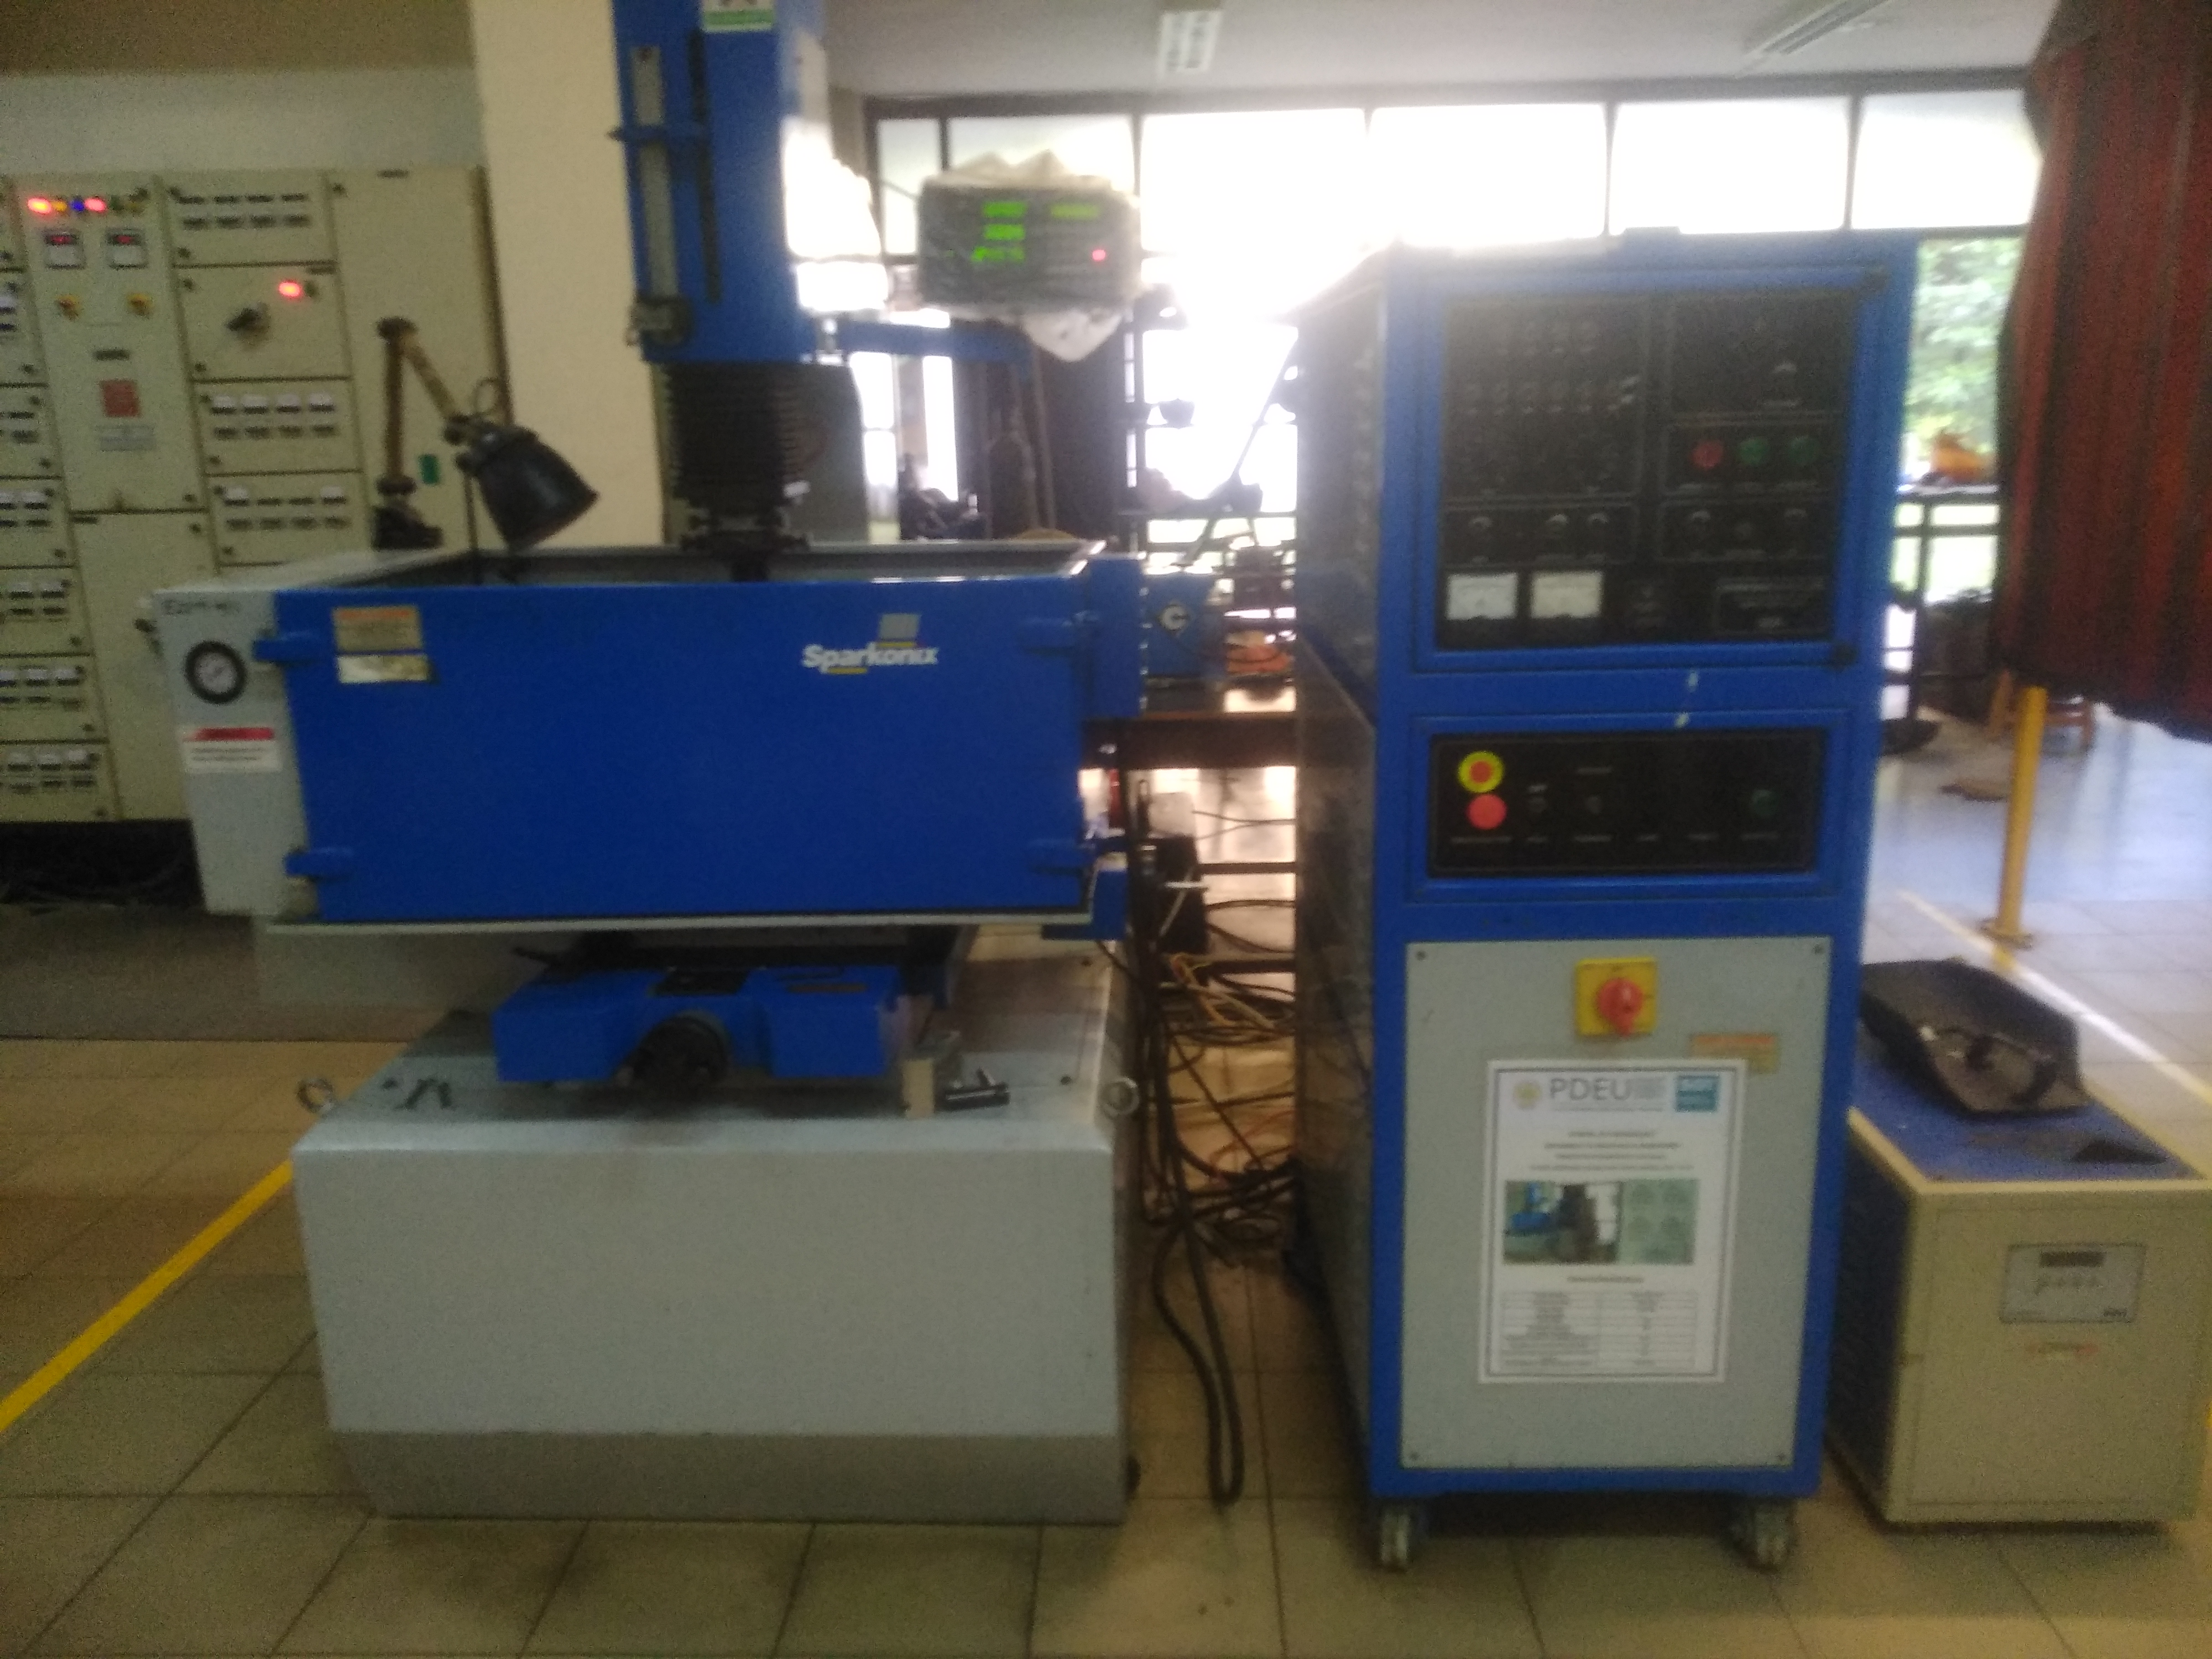
\includegraphics[width=0.7\linewidth]{MMP-Sparkonix.jpg}
            \caption{EDM machine - Sparkonix}
            \label{fig:sparkonix}
   \end{minipage}
  \end{figure}
 \begin{table}[htbp] 
     \begin{minipage}{0.4\textwidth}
     \centering
    \caption{Input parameters}
     \begin{tabular}{|l|l|l|l|l|l|}	
       \hline
		Design factors & Code & \multicolumn{3}{c|}{Levels} \\ 	\hline
		~ & ~ & -1 & 0 &1 \\ \hline
		Pulse on time(Ton)µs & A & 3 & 5 & 7 \\ \hline
		Pulse off time(Toff))µs & B & 2 & 4 & 6 \\ \hline
		Discharge Current(Ip)amp & C & 10 & 20 & 30 \\ \hline
       \end{tabular}
       \label{tab:input}
       \end{minipage}
 \end{table}  

\newpage 
\subsection {surface roughness measurement}
  Surface roughness of the specimens, made with different process parameters, are measured (Table \ref{tab:inputoutput})  using a profilometer of Mitsubishi model SJ-410 as shown in Figure \ref{fig:profilometer} sets of observations are obtained and the average values are computed for Ra, Rq, Rz, Rp, Rv 
\begin{figure}[htbp]
    \begin{minipage}{0.7\textwidth}
        \centering
        \includegraphics[width=0.7\textwidth]{MMP_profilometer_pdpu.jpg}
        \captionof{figure}{Profilometer-SJ410}
        \label{fig:profilometer}
    \end{minipage}
 \end{figure}
 \begin{table}[htbp]
    \centering
     \captionof{table}{ Process parameters and Roughness details of Specimens}
    \begin{tabular}{|l|l|l|l|l|l|l|l|l|}
    \hline
        No& Ton & Toff & Ip & Ra & Rq & Rz & Rp & Rv   \\ \hline
        1 & 3 & 2 & 10 & 4.252 & 5.585 & 28.935 & 12.071 & 16.865 \\ \hline
        2 & 3 & 2 & 20 & 4.442 & 5.664 & 26.886 & 10.423 & 16.462 \\ \hline
        3 & 3 & 2 & 30 & 5.428 & 6.928 & 29.213 & 14.856 & 14.356 \\ \hline
        4 & 3 & 4 & 10 & 4.317 & 5.309 & 24.604 & 10.612 & 13.992 \\ \hline
        5 & 3 & 4 & 20 & 4.489 & 5.518 & 25.57 & 10.429 & 14.141 \\ \hline
        6 & 3 & 4 & 30 & 5.061 & 6.529 & 29.292 & 13.338 & 15.954 \\ \hline
        7 & 3 & 6 & 10 & 4.047 & 5.047 & 23.099 & 9.117 & 13.982 \\ \hline
        8 & 3 & 6 & 20 & 4.372 & 5.399 & 23.959 & 12.019 & 11.94 \\ \hline
        9 & 3 & 6 & 30 & 4.681 & 5.705 & 23.789 & 10.131 & 13.658 \\ \hline
        10 & 5 & 2 & 10 & 4.296 & 5.735 & 27.909 & 14.507 & 13.402 \\ \hline
        11 & 5 & 2 & 20 & 4.706 & 6.136 & 27.858 & 11.558 & 16.3 \\ \hline
        12 & 5 & 2 & 30 & 5.077 & 6.45 & 29.005 & 12.618 & 16.388 \\ \hline
        13 & 5 & 4 & 10 & 4.506 & 5.695 & 25.707 & 9.887 & 15.82 \\ \hline
        14 & 5 & 4 & 20 & 4.761 & 5.803 & 25.066 & 10.824 & 14.242 \\ \hline
        15 & 5 & 4 & 30 & 5.561 & 6.807 & 28.956 & 13.056 & 15.9 \\ \hline
        16 & 5 & 6 & 10 & 4.742 & 5.915 & 26.665 & 12.601 & 14.064 \\ \hline
        17 & 5 & 6 & 20 & 4.864 & 6.344 & 27.857 & 11.205 & 16.651 \\ \hline
        18 & 5 & 6 & 30 & 6.48 & 8.296 & 35.502 & 18.892 & 16.61 \\ \hline
        19 & 7 & 2 & 10 & 3.936 & 4.971 & 22.736 & 9.606 & 13.13 \\ \hline
        20 & 7 & 2 & 20 & 4.278 & 5.611 & 27.583 & 15.535 & 12.048 \\ \hline
        21 & 7 & 2 & 30 & 5.007 & 6.013 & 25.309 & 11.77 & 13.539 \\ \hline
        22 & 7 & 4 & 10 & 4.133 & 5.202 & 24.117 & 11.084 & 13.033 \\ \hline
        23 & 7 & 4 & 20 & 4.389 & 5.409 & 24.965 & 10.593 & 14.372 \\ \hline
        24 & 7 & 4 & 30 & 5.177 & 6.337 & 26.83 & 10.833 & 15.997 \\ \hline
        25 & 7 & 6 & 10 & 4.746 & 5.719 & 25.865 & 10.565 & 15.3 \\ \hline
        26 & 7 & 6 & 20 & 5.016 & 6.19 & 27.16 & 11.631 & 15.53 \\ \hline
        27 & 7 & 6 & 30 & 5.274 & 6.357 & 27.608 & 11.603 & 16.004 \\ \hline
    \end{tabular}
    \label{tab:inputoutput}
\end{table}
\newpage
 \subsection{Development of model using  Arificial Neural Network (ANN) }

	A neural network is made up of a number of layers that each contain various components known as neurons. Network formation determines the network's type. Weights are used in the learning process to convert the network's storage of processing power. The training algorithm is a process that involves changing a network's weights to reduce a chosen function of error between the actual and desired outputs [1].
	Today's industrial applications use ANN.  ANN can be used in a variety of manufacturing processes. Input, hidden, and output layers make up its three primary layers. The input layer's neurons send information from the outside environment to the hidden layer.  Utilizing data from the input layer and the activation, bias, and summation functions, outputs are generated in the hidden layer. The ANN's workings are displayed in Figure \ref{fig:network}. The model is developed using Leven Berge-Marqardt algorithm with Adam optimizer. Convolutional Neural Networks (CNNs) are being trained by the authors to analyze and characterize the topology of a surface using the current methodology. The objective is to develop a method that can accurately assess surface topology using CNNs. This machine can generate surfaces with standard characteristics, which are essential for training the CNN models. By producing 
 \begin{figure}[htbp]
	\centering
	\includegraphics[width= 0.45\textwidth]{MMP_network.JPG}
	\caption{Neural Network}
   \label{fig:network}
\end{figure}
 surfaces with known characteristics, they can train the CNNs to accurately identify and characterize different surface topologies. The researchers aim to create a robust and versatile system that can analyze and classify surfaces based on their topology, regardless of the specific roughness average (Ra) value. This work has the potential to enhance the understanding and characterization of surfaces in various industries and applications[2]. 
  In the era of rapid development of science and technology, people’s requirements for intelligence are getting higher
and higher, and artificial intelligence has set off a new wave. Artificial neural networks (ANN) is a computational model
that mimics biological neural networks. It evolved from the single-layer perceptron M-P model proposed in 1943 to a
computing model that now has a multilayer perceptron network.13–16 The computational power is greatly improved and
can deal with complex nonlinear problems. It is widely used in model recognition, machine vision, speech recognition,
and other artificial intelligence fields. A BP neural network is a feed-forward artificial neural network using an error back
propagation algorithm, it has strong adaptive self-learning ability, superior fault tolerance, and robustness, and is the
most widely used of the neural network models. BP neural networks structure is divided into three layers, namely, the
input layer, hidden layer, and output layer, through the connection between each layer connection weights and threshold
values, as shown in Figure 1. The basic principle is that the input vector flows through the hidden layer and the output
layer of the inter-layer transfer function. If the demand is not met, the output value of the neuron is returned. The learning
process is modified by modifying the connection weight and threshold value. The whole process continues until the output
value meets the requirements and terminates.\cite{zhang2023prediction}

The following metrics, defined by equations 1,2 and 3, will be used for testing the efficacy of the prediction model. 

Mean Squared Error (MSE):
\begin{equation}
\mathrm{MSE} = \frac{1}{N} \sum_{i}\left|\mathrm{t}_{i}-\mathrm{o}_{i}\right|^{2}
\end{equation}

Mean Absolute Percentage Error (MAPE):
\begin{equation}
\mathrm{MAPE} = \frac{1}{N} \sum_{i}\left|\frac{t_{i}-o_{i}}{t_{i}}\right| \times 100
\end{equation}

R-squared (\( R^2 \)):
\begin{equation}
\mathrm{R^{2}} = 1 - \frac{\sum_{i}(\mathrm{t}_{i}-\mathrm{o}_{i})^{2}}{\sum_{i}(\mathrm{o}_{i})^{2}}
\end{equation}
\newpage 
\subsection{Prediction using Response Surface Method(RSM) }  
   Multiple regression is statistical technique to determine predicted values. In order to predict roughness parameters  $R_a$, $R_q$, $R_z$, $R_p$, $R_v$ Equation \ref{eq:equvar} is used.  
\begin{equation}
`				Y = \beta_0 + \sum_{i=1}^k \beta_i \cdot X_i + \sum_{i=1}^k \beta_{i i} \cdot X_i^2 + \sum_{j>1}^k \beta_{i j} \cdot X_i \cdot X_j + \varepsilon
            \label{eq:equvar}
\end{equation}
	where Y represents the corresponding response, i.e., $R_a$ of EDM process in the present work, 	$X_i$ is the input variables, $X_i^2$ and $X_i \cdot X_j$ are the squares and interaction terms, respectively, The influences of EDM parameters ($T_{on}$, $T_{off}$, $I_p$) on surface roughness ($R_a$) have been assessed for EN8 steel. The second-order model is the relationship between the surface roughness parameter and the 
 Multiple regression is a statistical technique that allows us to determine the correlation between a continuous dependent variable and two or more continuous or discrete independent variables. 

 Results obtained by using RSM model will be elaborated in section 4.1. 
 

   
   

 \section{\fontsize{14}{18}\selectfont\textbf{Results and Discussion}}
 \subsection{\textbf{ANOVA and regression equation of Ra}}
  ANOVA technique helps in identifying the most influencing factor affecting the output parameter(Ra).The technique uses sum of squares and variance during analysis. Least squares technique is used in this approach. Table 4 shows the input factor levels and input values 

 Table \ref{tab:rsmRv} shows the variance of analysis for Ra. 
 

\begin{table}[!ht]
    \centering
      \caption{Variace analysis for Ra}
    \begin{tabular}{|l|l|l|l|l|l|}
    \hline
       Source & DF & Adj SS & Adj MS & F-Value & P-Val \\ \hline
        Model & 9 & 6.63904 & 0.73767 & 10.59 & 0 \\ \hline
        Linear & 3 & 4.75123 & 1.58374 & 22.73 & 0 \\ \hline
        Ton & 1 & 0.04176 & 0.04176 & 0.6 & 0.449 \\ \hline
        Toff & 1 & 0.43556 & 0.43556 & 6.25 & 0.023 \\ \hline
         Ip & 1 & 4.27391 & 4.27391 & 61.34 & 0 \\ \hline
        Square & 3 & 1.21507 & 0.40502 & 5.81 & 0.006 \\ \hline
        Ton*Ton & 1 & 0.89218 & 0.89218 & 12.8 & 0.002 \\ \hline
        Toff*Toff & 1 & 0.01357 & 0.01357 & 0.19 & 0.665 \\ \hline
        Ip*Ip & 1 & 0.30933 & 0.30933 & 4.44 & 0.05 \\ \hline
        2-Way & 3 & 0.67274 & 0.22425 & 3.22 & 0.049 \\ \hline
        Ton*Toff & 1 & 0.67071 & 0.67071 & 9.63 & 0.006 \\ \hline
        Ton*Ip & 1 & 0.00066 & 0.00066 & 0.01 & 0.924 \\ \hline
        Toff*Ip & 1 & 0.00137 & 0.00137 & 0.02 & 0.89 \\ \hline
        Error & 17 & 1.18447 & 0.06967 &    &    \\ \hline
        Total & 26 & 7.82351 &    &    &    \\ \hline
    \end{tabular}
    \label{tab:rsmRv}
\end{table}
\newpage
The surface parameters (Ra) is predicted using input values of Ton, Toff, Ip 

\begin{align}
\begin{split}
R_a = &\, 3.27 + 0.744 \cdot \text{Ton} - 0.302 \cdot \text{Toff} - 0.0418 \cdot \text{Ip} \\
&- 0.0964 \cdot \text{Ton}^2 + 0.0119 \cdot \text{Toff}^2 + 0.00227 \cdot \text{Ip}^2 \\
&+ 0.0591 \cdot \text{Ton} \cdot \text{Toff} + 0.00037 \cdot \text{Ton} \cdot \text{Ip} - 0.00053 \cdot \text{Toff} \cdot \text{Ip}
\end{split}
\label{eq:Reqv}
\end{align}
\subsection{RSM surface plots}

Figure \ref{fig:ToffTon} shows that as value of Ton increases Ra is increased but the increase is not significant,where  as it is significant when value of Toff is increased
  %  \begin{minipage}{0.7\textwidth}
  \begin{figure}[htbp]
    \centering
    \includegraphics[width=\textwidth]{MMP_3D_Ra_Toff_Ton.jpg}
    \captionof{figure}{3D Plot Ra v/s Toff,Ton}
    \label{fig:ToffTon}
  \end{figure}
 % \begin{minipage}{1\textwidth}
 
 Figure \ref{fig:IpTon} shows that as value of Ton increases Ra is increased but the increase is not significant,where  as it is significant when value of Ip is increased
 \begin{figure}[htbp]
    \centering
    \includegraphics[width=\textwidth]{MMP_3D_Ra_Ip_Ton.jpg}
    \captionof{figure}{3D Plot of Ra v/s Ton, Ip}
  \label{fig:IpTon}
  \end{figure}

   Figure \ref{fig:IpToff} shows that as value of Toff increases Ra is not  increasing significantly. when value of Ip is increasing  Ra is also increasing fast. It indicates that value of peak current affects surface roughness Ra significantly.
  \begin{minipage}{1\textwidth}
    \centering
    \includegraphics[width=\linewidth]{Ra-Toff,Ip.jpg}
  \captionof{figure}{3D Plot of Ra v/s Toff, Ip}
    \label{fig:IpToff}
  \end{minipage}
  \hfill
 
 
   Figure \ref{fig:RSM_comp_line} is bar chart of comparison of actual Ra-values and predicted Ra values. both the values are in proximity, showing strength of RSM model. 
  \begin{minipage}{1\textwidth}
     \centering
    \includegraphics[width=\textwidth]{comp_Ra_pRa.jpg}
    \captionof{figure}{Comarative graph of RSM for actual and predicted vaues of surface roughness}
    \label{fig:RSM_comp_line}
  \end{minipage}
  % \hfill
  % \begin{minipage}{1\textwidth}
  %   \centering
  %   \includegraphics[width=\textwidth]{MMP_LM_test.jpg}
  %   \captionof{figure}{R$^2$ value of LM optimizer}
  % \label{fig:Ion}
  % \end{minipage}
  \newpage
    Figure \ref{fig}  
\subsection{ Response surface method (RSM) results}
     \begin{minipage}{1\textwidth}
       \small
         \captionof{table}{RSM Results}
        \begin{tabular}{|p{1.2em}|p{1.2em}|p{1.2em}|l|l|l|l|l|l|l|l|l|l|l|l|l|}  \hline  
         Exp & \multicolumn{3}{l|}{Input factors} & \multicolumn{5}{l|}{ Experiment Output variables}&\multicolumn{5}{l|}{ Predicted output variables}\\ \hline
        No& Ton & Toff & Ip & Ra & Rq & Rz & Rp & Rv  & pRa & pRq & pRz & pRp & pRv  \\ \hline
        1 & 3 & 2 & 10 & 4.252 & 5.585 & 28.935 & 12.071 & 16.865 & 4.247 & 5.527 & 27.770 & 11.700 & 16.042 \\ \hline
        2 & 3 & 2 & 20 & 4.442 & 5.664 & 26.886 & 10.423 & 16.462 & 4.511 & 5.834 & 27.860 & 12.020 & 15.693 \\ \hline
        3 & 3 & 2 & 30 & 5.428 & 6.928 & 29.213 & 14.856 & 14.356 & 5.228 & 6.636 & 29.200 & 13.300 & 15.857 \\ \hline
        4 & 3 & 4 & 10 & 4.317 & 5.309 & 24.604 & 10.612 & 13.992 & 4.130 & 5.117 & 24.420 & 9.640 & 14.627 \\ \hline
        5 & 3 & 4 & 20 & 4.489 & 5.518 & 25.570 & 10.429 & 14.141 & 4.382 & 5.472 & 25.110 & 10.400 & 14.448 \\ \hline
        6 & 3 & 4 & 30 & 5.061 & 6.529 & 29.292 & 13.338 & 15.954 & 5.089 & 6.323 & 27.060 & 12.130 & 14.783 \\ \hline
        7 & 3 & 6 & 10 & 4.047 & 5.047 & 23.099 & 9.117 & 13.982 & 4.107 & 5.023 & 22.920 & 9.740 & 13.138 \\ \hline
        8 & 3 & 6 & 20 & 4.372 & 5.399 & 23.959 & 12.019 & 11.940 & 4.349 & 5.427 & 24.220 & 10.950 & 13.129 \\ \hline
        9 & 3 & 6 & 30 & 4.681 & 5.705 & 23.789 & 10.131 & 13.658 & 5.045 & 6.325 & 26.780 & 13.110 & 13.633 \\ \hline
        10 & 5 & 2 & 10 & 4.296 & 5.735 & 27.909 & 14.507 & 13.402 & 4.437 & 5.863 & 28.190 & 13.100 & 15.170 \\ \hline
        11 & 5 & 2 & 20 & 4.706 & 6.136 & 27.858 & 11.558 & 16.300 & 4.708 & 6.137 & 28.390 & 13.120 & 15.233 \\ \hline
        12 & 5 & 2 & 30 & 5.077 & 6.450 & 29.005 & 12.618 & 16.388 & 5.433 & 6.905 & 29.850 & 14.110 & 15.810 \\ \hline
        13 & 5 & 4 & 10 & 4.506 & 5.695 & 25.707 & 9.887 & 15.820 & 4.556 & 5.761 & 26.430 & 11.290 & 15.107 \\ \hline
        14 & 5 & 4 & 20 & 4.761 & 5.803 & 25.066 & 10.824 & 14.242 & 4.816 & 6.083 & 27.240 & 11.750 & 15.340 \\ \hline
        15 & 5 & 4 & 30 & 5.561 & 6.807 & 28.956 & 13.056 & 15.900 & 5.530 & 6.900 & 29.310 & 13.180 & 16.087 \\ \hline
        16 & 5 & 6 & 10 & 4.742 & 5.915 & 26.665 & 12.601 & 14.064 & 4.770 & 5.976 & 26.530 & 11.640 & 14.969 \\ \hline
        17 & 5 & 6 & 20 & 4.864 & 6.344 & 27.857 & 11.205 & 16.651 & 5.019 & 6.346 & 27.950 & 12.540 & 15.372 \\ \hline
        18 & 5 & 6 & 30 & 6.480 & 8.296 & 35.502 & 18.892 & 16.610 & 5.723 & 7.210 & 30.630 & 14.410 & 16.289 \\ \hline
        19 & 7 & 2 & 10 & 3.936 & 4.971 & 22.736 & 9.606 & 13.130 & 3.856 & 4.992 & 23.990 & 11.820 & 12.248 \\ \hline
        20 & 7 & 2 & 20 & 4.278 & 5.611 & 27.583 & 15.535 & 12.048 & 4.134 & 5.232 & 24.310 & 11.550 & 12.723 \\ \hline
        21 & 7 & 2 & 30 & 5.007 & 6.013 & 25.309 & 11.770 & 13.539 & 4.867 & 5.966 & 25.880 & 12.240 & 13.712 \\ \hline
        22 & 7 & 4 & 10 & 4.133 & 5.202 & 24.117 & 11.084 & 13.033 & 4.211 & 5.198 & 23.840 & 10.260 & 13.536 \\ \hline
        23 & 7 & 4 & 20 & 4.389 & 5.409 & 24.965 & 10.593 & 14.372 & 4.479 & 5.486 & 24.760 & 10.430 & 14.182 \\ \hline
        24 & 7 & 4 & 30 & 5.177 & 6.337 & 26.830 & 10.833 & 15.997 & 5.200 & 6.269 & 26.940 & 11.560 & 15.341 \\ \hline
        25 & 7 & 6 & 10 & 4.746 & 5.719 & 25.865 & 10.565 & 15.300 & 4.661 & 5.721 & 25.540 & 10.860 & 14.750 \\ \hline
        26 & 7 & 6 & 20 & 5.016 & 6.190 & 27.160 & 11.631 & 15.530 & 4.918 & 6.057 & 27.070 & 11.470 & 15.566 \\ \hline
        27 & 7 & 6 & 30 & 5.274 & 6.357 & 27.608 & 11.603 & 16.004 & 5.629 & 6.888 & 29.860 & 13.040 & 16.895 \\ \hline
    \end{tabular}
    \label{tab:output}
    \end{minipage} 

\begin {itemize}
\item The two-stage effort of obtaining a Surface Roughness (SR) model by RSM and optimization of this model,
have resulted in a fairly useful method of obtaining process parameters in order to attain the improved
surface quality.
\item  The investigation indicates that the discharge current, pulse-on time and pulse-off time are the primary factors influencing the SR of EDM8 material during EDM machining.
\item  Pulse-on time is found to be the dominant parameter influencing surface roughness.
\item An increase in discharge current(Ip) was also observed to increase the roughness of the surface. The confirmation test showed that developed models can predict the SR accurately within 95\% confidence interval.
\item  The methodology adopted establishes the optimization and hence facilitates the effective use of EDM machinable EN8 in industrial applications.
\end{itemize}
Results of RSM method are summarised in Table \ref{tab:rsmmaper2} for R$^2$ and 100-MAPE. It is observed that values are comparatively lower than that in Table \ref{tab:annmaper2}

\begin{table}[htbp]
   \caption{ RSM method - Results of 100-MAPE and R$^2$} 
    \hspace{-8em}
    \small
    \begin{tabular}{|c|l|l|l|l|l|l|l|l|l||l|}
    \hline
        ~ & \multicolumn{5}{c|}{100-MAPE}& \multicolumn{5}{c|}{R$^2$}  \\ \hline
         Surface roughness & Ra & Rq & Rz & Rp & Rv & Ra &    Rq & Rz & Rp & Rv \\ \hline
         RSM               & 97.2563 & 97.0520 & 96.4014 & 89.6507 & 94.9921 & 99.8075 & 99.7379 & 99.6679 & 98.1065 & 99.6734\\ \hline
    \end{tabular}
    \label{tab:rsmmaper2}
\end{table}
\subsection{Artificial Neural Network results : MSE, 100-MAPE, R$^2$, using GD, GDA, LM, RP optimizers for Ra,Rq,Rz,Rp,Rv roughness characterization }	
\subsubsection{ Levenberg Marquadt (LM) -  Rv} 
 \begin{minipage}{0.40\textwidth}
  \small
 \centering
 \captionof{table}{ MSE - Training}
    \begin{tabular}{|c|c|c|c|c|c|}
    \hline
        Model & Ra &  Rq &  Rz &  Rp & Rv \\ \hline
        3,3,5 & 0.6145 & 0.5268 & 12.7484 & 5.7805 & 1.9906 \\ \hline
        3,4,5 & 0.2320 & 0.3116 & 5.7632 & 3.3648 & 1.5589 \\ \hline
        3,5,5 & 0.2577 & 0.3769 & 5.6313 & 4.1938 & 1.6742 \\ \hline
        3,6,5 & 0.2611 & 0.3980 & 5.8941 & 4.3860 & 1.7359 \\ \hline
        3,7,5 & 0.3598 & 0.3524 & 5.1894 & 3.7249 & 1.7618 \\ \hline
        3,8,5 & 0.4466 & 0.5745 & 9.0193 & 5.1845 & 2.2094 \\ \hline
        3,9,5 & 0.2267 & 0.4160 & 4.8924 & 3.4021 & 1.7225 \\ \hline
        3,10,5 & 0.5112 & 0.5755 & 6.4854 & 5.1552 & 2.1182 \\ \hline
    \end{tabular}
        \label{tab:lmmsetr}
    \end{minipage}
    \hfill 
     \begin{minipage}{0.38\textwidth} 
   \small
 \centering
 \captionof{table}{MSE - Testing}
    \begin{tabular}{|c|c|c|c|c|c|}
    \hline
        Ra &  Rq &  Rz &  Rp & Rv \\ \hline
         0.8816 & 0.6776 & 13.3610 & 10.9872 & 1.7374 \\ \hline
         0.2875 & 0.5838 & 11.6035 & 7.7585 & 2.7788 \\ \hline
         0.2320 & 0.4469 & 15.8244 & 7.5464 & 2.8476 \\ \hline
         0.3246 & 0.5137 & 7.2145 & 4.4629 & 2.7386 \\ \hline
         0.3732 & 0.4807 & 9.1344 & 5.6403 & 1.9395 \\ \hline
         0.4320 & 0.6740 & 10.2400 & 7.4878 & 2.7025 \\ \hline
         0.3072 & 0.4975 & 9.3864 & 5.9403 & 2.4214 \\ \hline
         0.3583 & 0.5034 & 8.1824 & 5.4917 & 2.6757 \\ \hline
    \end{tabular}
        \label{tab:lmmsete}
    \end{minipage}
    \hfill
    \begin{minipage}{0.40\textwidth}
   \small
\centering
 \captionof{table}{100-MAPE - Training}
      \begin{tabular}{|c|c|c|c|c|c|}
    \hline
         Model & Ra &  Rq &  Rz &  Rp & Rv \\ \hline
         3,3,5 &89.4593 & 91.3179 & 91.4111 & 86.4767 & 92.1775 \\ \hline
         3,4,5 &92.3164 & 93.3200 & 93.5700 & 88.9384 & 93.3983 \\ \hline
        3,5,5 & 91.9950 & 92.3777 & 94.0158 & 88.5328 & 93.2417 \\ \hline
         3,6,5 &91.7527 & 92.0989 & 93.2501 & 88.1002 & 92.2379 \\ \hline
        3,7,5 & 90.5230 & 93.0120 & 94.3972 & 89.7952 & 92.1567 \\ \hline
         3,8,5 &88.6511 & 90.5537 & 91.5667 & 86.1443 & 92.1446 \\ \hline
        3,9,5 & 92.6582 & 91.9939 & 94.3163 & 89.5222 & 92.6677 \\ \hline
         3,10,5 &90.0553 & 90.5693 & 92.9260 & 87.0656 & 91.6169 \\ \hline
    \end{tabular}
        \label{tab:lmmapetr}
    \end{minipage}
    \hfill 
     \begin{minipage}{0.33\textwidth}
   \small
\captionof{table}{\makebox[2.2cm][l]{ 100-MAPE-Testing}}
     \begin{tabular}{|c|c|c|c|c|}
    \hline
         Ra &  Rq &  Rz &  Rp & Rv \\ \hline
        86.7293 & 89.5728 & 90.0064 & 79.0522 & 92.7297 \\ \hline
        91.4049 & 90.9243 & 90.6595 & 83.7028 & 90.0244 \\ \hline
        92.2612 & 91.4242 & 89.8107 & 84.6160 & 90.1505 \\ \hline
        90.8824 & 91.6115 & 92.6710 & 87.6929 & 90.5660 \\ \hline
        89.8605 & 91.7290 & 91.8469 & 86.2687 & 91.4846 \\ \hline
        88.2478 & 88.5413 & 89.9262 & 80.5972 & 90.4051 \\ \hline
        91.4528 & 90.9285 & 91.0559 & 85.6070 & 90.6770 \\ \hline
        90.7455 & 92.0504 & 91.6534 & 87.3093 & 90.2720 \\ \hline
    \end{tabular}
        \label{tab:lmmapete}
    \end{minipage}
     \begin{minipage}{0.40\textwidth}
        \small
 \centering
 \captionof{table}{R$^2$ - Training}
    \begin{tabular}{|c|c|c|c|c|c|}
    \hline
      model & Ra &  Rq &  Rz &  Rp & Rv \\ \hline
    3,3,5 & 97.3125 & 98.5430 & 98.2424 & 96.0009 & 99.1047 \\ \hline
       3,4,5 & 98.9802 & 99.1304 & 99.2027 & 97.7187 & 99.2958 \\ \hline
        3,5,5 &98.8711 & 98.9524 & 99.2246 & 97.1506 & 99.2439 \\ \hline
        3,6,5 &98.8594 & 98.8940 & 99.1891 & 97.0186 & 99.2130 \\ \hline
        3,7,5 &98.4280 & 99.0220 & 99.2810 & 97.4483 & 99.2045 \\ \hline
        3,8,5 &98.0326 & 98.3923 & 98.7486 & 96.4500 & 98.9990 \\ \hline
        3,9,5 &99.0059 & 98.8388 & 99.3193 & 97.6813 & 99.2155 \\ \hline
        3,10,5 &97.7623 & 98.4061 & 99.1010 & 96.4899 & 99.0421 \\ \hline
    \end{tabular}
        \label{tab:lmr2tr}
    \end{minipage}
    \hfill 
    \begin{minipage}{0.33\textwidth}
    \small
 \centering
 \captionof{table}{R$^2$ - Testing}
    \begin{tabular}{|c|c|c|c|c|c|}
    \hline
        Ra &  Rq &  Rz &  Rp & Rv \\ \hline
        96.1432 & 98.1774 & 98.1592 & 92.4814 & 99.2417 \\ \hline
        98.7373 & 98.3834 & 98.4129 & 94.8385 & 98.7364 \\ \hline
        99.0192 & 98.7908 & 97.8311 & 95.0236 & 98.7175 \\ \hline
        98.6094 & 98.6718 & 99.0452 & 97.1497 & 98.7152 \\ \hline
        98.4467 & 98.7549 & 98.7688 & 96.4110 & 99.1228 \\ \hline
        98.1316 & 98.1550 & 98.5770 & 94.9701 & 98.7780 \\ \hline
        98.7123 & 98.6582 & 98.7163 & 96.1578 & 98.8921 \\ \hline
        98.4620 & 98.6382 & 98.8616 & 96.5370 & 98.7453 \\ \hline
     \end{tabular}
     \label{tab:lmr2te}
     \end{minipage}
     
     Table  \begin{table}[hbtp]
   \fontsize{8}{9}
    \caption{Comparison of results of optimizers}
     \hspace{-8em}
    \begin{tabular}{|l|*{5}{c|}*{5}{c|}}   \hline
         ~ & \multicolumn{5}{c|}{Maximum value of-(100-MAPE)} & \multicolumn{5}{c|}{Maximum value of-R$^2$}  \\ \hline
        Optimizer &   Ra &   Rq &   Rz &   Rp &   Rv &    Ra &   Rq &   Rz &   Rp   &  Rv \\ \hline
        \multirow{2}{*}{\shortstack{GD-Train \\ Architecture}} & 89.6233 & 90.9756 & \multirow{2}{*}{\shortstack{\textit{\textbf{95.1854}} \\ (3,4,5)}} & \multirow{2}{*}{\shortstack{\textit{\textbf{90.1051}} \\ (3,7,5)}}& 92.8531 &  98.3436 & 98.5673 & \multirow{2}{*}{\shortstack{\textit{\textbf{99.4371}} \\ (3,7,5)}} & \multirow{2}{*}{\shortstack{\textit{\textbf{97.8093}} \\ (3,7,5)}} & 99.2045 \\  & & & & & & & & & & \\\hline
        \multirow{2}{*}{\shortstack{GD-Test \\ Architecture}} &  89.1217 & 90.7939 & \multirow{2}{*}{\shortstack{ \textit{\textbf{93.5771}} \\ (3,8,5)}} & 88.2682 & 92.4535  & 98.2255 & 98.4715 & \multirow{2}{*}{\shortstack{\textit{\textbf{99.3314}} \\ (3,7,5)}} & 97.1350 & 99.1621 \\  & & & & & & & & & & \\ \hline
        GDA-Train & 90.1563 & 91.7614 & 93.7724 & 88.5534 & 91.6212 & 98.5452 & 98.7759 & 99.2662 & 97.4794 & 99.1045 \\ \hline
        \multirow{2}{*}{\shortstack{GDA-Test \\ Architecture}} & 90.8329 & 92.0182 & 92.8793 & 89.4264 & 91.2591  & 98.6352 & \multirow{2}{*}{\shortstack{\textit{\textbf{98.8806}} \\ (3,9,5)}}& 99.1269 & 97.1419 & 98.9789 \\  & & & & & & & & & & \\ \hline
        
         \multirow{2}{*}{\shortstack{LM-Train \\ Architecture}} &\multirow{2}{*}{\shortstack{\textit{\textbf{92.6582}}  \\ (3,9,5)}} & \multirow{2}{*}{\shortstack{\textit{\textbf{93.3200}} \\ (3,4,5) }} &  94.3972  & 89.7952 &  \multirow{2}{*}{\shortstack{\textit{\textbf{93.3983}} \\ (3,4,5)}}   & \multirow{2}{*}{\shortstack{\textit{\textbf{99.0059}} \\ (3,9,5)}} & \multirow{2}{*}{\shortstack{\textit{\textbf{99.1304}} \\ (3,4,5)}} & 99.3193 & 97.7187 & \multirow{2}{*}{\shortstack{\textit{\textbf{99.2958}} \\ (3,4,5)}} \\ & & & & & & & & & & \\  \hline 
        \multirow{2}{*}{\shortstack{LM-Test \\ Architecture }}  & \multirow{2}{*}{\shortstack{\textit{\textbf{92.2612}} \\ (3,5,5)}} & \multirow{2}{*}{\shortstack{\textit{\textbf{92.0504}} \\ (3,10,5)}} & 92.6710 & 86.2687 & \multirow{2}{*}{\shortstack{\textit{\textbf{92.7297}} \\ (3,3,5)}}  & \multirow{2}{*}{\shortstack{\textit{\textbf{99.0192}} \\ (3,5,5)}} & 98.7908 & 99.0452 & 97.1497 & \multirow{2}{*}{\shortstack{\textit{\textbf{99.2417}} \\ (3,3,5)}} \\ & & & & & & & & & & \\\hline
        RP-Train & 91.7322 & 92.3465 & 94.2465 & 89.8786 & 92.0171 & 98.8003 & 98.9374 & 99.3242 & 97.7675 & 99.2058 \\ \hline
        \multirow{2}{*}{\shortstack{RP -Test \\ Architecture}} & 90.5510 & 91.5441 & 92.5949 & \multirow{2}{*}{\shortstack{\textit{\textbf{88.5802}} \\ (3,4,5)}}& 91.5324  & 98.3773 & 98.3773 & 99.1112 & \multirow{2}{*}{\shortstack{\textit{\textbf{97.2680}} \\ (3,4,5)}}& 99.1168 \\ & & & & & & & & & & \\ \hline
   \end{tabular}
   \label{tab:annmaper2}
\end{table}
\newpage
\section{Conclusion}\label{sec:concl}

It is concluded from the results that the Leven Berg-Marquardt (LM) algorithm  has an accuracy using Training and testing results of MAPE and R$2$ is around 92\% and 97\% respectively for surface roughness  Ra,Rq and Rv while Rz follows Gradient Descent (GD)  and Root mean squared Prop (RP) follows partialy GD and RP algorithms.The study proposes a deep learning-based method employing images of die-sinking EDM-machined work piece surfaces.Looking at these pictures captured by a CCD  camera, the recommended method may accurately predict surface roughness values comparable to those acquired by a profilometer. With the help of this integrated technique, operators can measure roughness values that correspond to goal specifications on designs. Additionally, the learning-based technique shows promise for characterizing surface morphology and enabling automatic in-situ quality control in intelligent manufacturing cells, applicable to both EDM machining and other machining processes.

\bibliographystyle{unsrt}
\bibliography{MMP_cite} 

%\begin{verbatim}
\section{ Supplementary information}
\subsection{Declaration}
\begin{itemize}
\item The authors have no relevant financial or non-financial interests to disclose.
\item The authors have no conflicts of interest to declare that are relevant to the content of this article.
\item All authors certify that they have no affiliations with or involvement in any organization or entity with any financial interest or non-financial interest in the subject matter or materials discussed in this manuscript.
\item The authors have no financial or proprietary interest in the material discussed in this article.
\end{itemize}
\subsubsection {Funding}
The authors did not receive funding from any organization for the submitted work. Also, the authors declare they have no financial interests. Therefore, the authors have no relevant financial or non-financial interests to disclose.
\subsubsection{Conflicts of interest/Competing interests}
There are not any Conflicts of interest and Competing interests about the presented results in this paper. All results are based on laboratory data and based on common statistical criteria in the scientific articles.
.
0
\subsection{Availability of data and material}
All of data and material are presented in Figures
\subsubsection{Code availability}
\begin{landscape}
\section { Annexure :  I}
 \begin{minipage}{0.50\textwidth}
\centering
 \captionof{table}{ANOVA - Rv}
    \centering
\begin{tabular}{|l|l|l|l|l|l|}
    \hline
      Source & DF & Adj SS & Adj MS & F-Value & P-Value \\ \hline
        Model & 9 & 38.4628 & 4.2736 & 4.64 & 0.004 \\ \hline
        Linear & 3 & 2.4327 & 0.8109 & 0.88 & 0.472 \\ \hline
        Ton & 1 & 0.3192 & 0.3192 & 0.35 & 0.564 \\ \hline
        Toff & 1 & 0.1063 & 0.1063 & 0.12 & 0.739 \\ \hline
        Ip & 1 & 1.9239 & 1.9239 & 2.09 & 0.168 \\ \hline
        Square & 3 & 10.1324 & 3.3775 & 3.66 & 0.035 \\ \hline
        Ton*Ton & 1 & 9.4514 & 9.4514 & 10.25 & 0.006 \\ \hline
        Toff*Toff & 1 & 0.0732 & 0.0732 & 0.08 & 0.782 \\ \hline
        Ip*Ip & 1 & 0.9629 & 0.9629 & 1.04 & 0.322 \\ \hline
        2-Way Interaction & 3 & 25.6187 & 8.5396 & 9.26 & 0.001 \\ \hline
        Ton*Toff & 1 & 21.924 & 21.924 & 23.78 & 0 \\ \hline
        Ton*Ip & 1 & 2.0402 & 2.0402 & 2.21 & 0.156 \\ \hline
        Toff*Ip & 1 & 1.6544 & 1.6544 & 1.79 & 0.199 \\ \hline
        Error & 16 & 14.7494 & 0.9218 & ~ & ~ \\ \hline
        Total & 25 & 53.2122 & ~ & ~ & ~ \\ \hline
       
    \end{tabular}
    \label{tab:annovaRa}
 \end{minipage}
    \hfill 
     \begin{minipage}{0.70\textwidth}
\centering
 \captionof{table}{ANOVA - Rq}
    \centering
    \centering
    \begin{tabular}{|l|l|l|l|l|l|}
    \hline
        Model & 9 & 9.9123 & 1.10136 & 7.37 & 0 \\ \hline
        Linear & 3 & 6.027 & 2.009 & 13.45 & 0 \\ \hline
        Ton & 1 & 0.0009 & 0.00087 & 0.01 & 0.94 \\ \hline
        Toff & 1 & 0.1961 & 0.19615 & 1.31 & 0.268 \\ \hline
        Ip & 1 & 5.83 & 5.82997 & 39.04 & 0 \\ \hline
        Square & 3 & 2.7048 & 0.90161 & 6.04 & 0.005 \\ \hline
        Ton*Ton & 1 & 2.1877 & 2.18769 & 14.65 & 0.001 \\ \hline
        Toff*Toff & 1 & 0.1501 & 0.1501 & 1.01 & 0.33 \\ \hline
        Ip*Ip & 1 & 0.367 & 0.36704 & 2.46 & 0.135 \\ \hline
        2-Way Interaction & 3 & 1.1805 & 0.39349 & 2.63 & 0.083 \\ \hline
        Ton*Toff & 1 & 1.139 & 1.13898 & 7.63 & 0.013 \\ \hline
        Ton*Ip & 1 & 0.0137 & 0.01374 & 0.09 & 0.765 \\ \hline
        Toff*Ip & 1 & 0.0277 & 0.02774 & 0.19 & 0.672 \\ \hline
        Error & 17 & 2.539 & 0.14935 & ~ & ~ \\ \hline
        Total & 26 & 12.4512 & ~ & ~ & ~ \\ \hline
    \end{tabular}
 \end{minipage}
    \hfill    
\begin{subequations}
\begin{minipage}{0.5\linewidth}
\begin{align}
\begin{split}
R_v = &\, 19.45 + 1.48 \cdot \text{Ton} - 2.348 \cdot \text{Toff} - 0.310 \cdot \text{Ip} \\
&- 0.331 \cdot \text{Ton}^2 + 0.0280 \cdot \text{Toff}^2 + 0.00406 \cdot \text{Ip}^2 \\
&+ 0.3379 \cdot \text{Ton} \cdot \text{Toff} + 0.0206 \cdot \text{Ton} \cdot \text{Ip} + 0.0197 \cdot \text{Toff} \cdot \text{Ip}
\end{split}
\label{eq:eqRa}
\end{align}
\end{minipage}
\hfill
\begin{minipage}{0.5\linewidth}
\begin{align}
\begin{split}
R_q = &\, 4.13 + 1.239 \cdot \text{Ton} - 0.697 \cdot \text{Toff} - 0.0432 \cdot \text{Ip} \\
&- 0.1510 \cdot \text{Ton}^2 + 0.0395 \cdot \text{Toff}^2 + 0.00247 \cdot \text{Ip}^2 \\
&+ 0.0770 \cdot \text{Ton} \cdot \text{Toff} - 0.00169 \cdot \text{Ton} \cdot \text{Ip} + 0.00240 \cdot \text{Toff} \cdot \text{Ip}
\end{split}
\label{eq:eqRb}
\end{align}
\end{minipage}
\end{subequations}
\end{landscape}
\begin{landscape}
 \begin{minipage}{0.50\textwidth}
\centering
 \captionof{table}{ANOVA - Rz}
    \centering
 \begin{tabular}{|l|l|l|l|l|l|}
    \hline
        Source & DF & Adj SS & Adj MS & F-Value & P-Value \\ \hline
        Model & 9 & 113.408 & 12.6009 & 3.31 & 0.016 \\ \hline
        Linear & 3 & 38.59 & 12.8633 & 3.38 & 0.043 \\ \hline
        Ton & 1 & 0.56 & 0.5597 & 0.15 & 0.706 \\ \hline
        Toff & 1 & 0.858 & 0.8581 & 0.23 & 0.641 \\ \hline
        Ip & 1 & 37.172 & 37.1723 & 9.76 & 0.006 \\ \hline
        Square & 3 & 39.498 & 13.1659 & 3.46 & 0.04 \\ \hline
        Ton*Ton & 1 & 31.94 & 31.9396 & 8.38 & 0.01 \\ \hline
        Toff*Toff & 1 & 5.179 & 5.1795 & 1.36 & 0.26 \\ \hline
        Ip*Ip & 1 & 2.378 & 2.3785 & 0.62 & 0.44 \\ \hline
        2-Way Interaction & 3 & 35.32 & 11.7735 & 3.09 & 0.055 \\ \hline
        Ton*Toff & 1 & 30.694 & 30.6944 & 8.06 & 0.011 \\ \hline
        Ton*Ip & 1 & 0.157 & 0.1571 & 0.04 & 0.841 \\ \hline
        Toff*Ip & 1 & 4.469 & 4.4689 & 1.17 & 0.294 \\ \hline
        Error & 17 & 64.768 & 3.8099 & ~ & ~ \\ \hline
        Total & 26 & 178.176 & ~ & ~ & ~ \\ \hline
    \end{tabular}
    \label{tab:annovaRz}
 \end{minipage}
    \hfill 
     \begin{minipage}{0.70\textwidth}
\centering
 \captionof{table}{ANOVA - Rp}
    \centering
    \centering
     \begin{tabular}{|l|l|l|l|l|l|}
    \hline
        Source & DF & Adj SS & Adj MS & F-Value & P-Value \\ \hline
        Model & 9 & 40.874 & 4.5416 & 1.03 & 0.453 \\ \hline
        Linear & 3 & 17.638 & 5.8793 & 1.34 & 0.295 \\ \hline
        Ton & 1 & 0.003 & 0.0028 & 0 & 0.98 \\ \hline
        Toff & 1 & 1.491 & 1.4907 & 0.34 & 0.568 \\ \hline
        Ip & 1 & 16.144 & 16.1445 & 3.68 & 0.072 \\ \hline
        Square & 3 & 19.111 & 6.3702 & 1.45 & 0.263 \\ \hline
        Ton*Ton & 1 & 10.738 & 10.7379 & 2.45 & 0.136 \\ \hline
        Toff*Toff & 1 & 6.967 & 6.9668 & 1.59 & 0.225 \\ \hline
        Ip*Ip & 1 & 1.406 & 1.4059 & 0.32 & 0.579 \\ \hline
        2-Way Interaction & 3 & 4.126 & 1.3753 & 0.31 & 0.816 \\ \hline
        Ton*Toff & 1 & 0.736 & 0.7356 & 0.17 & 0.687 \\ \hline
        Ton*Ip & 1 & 1.064 & 1.0645 & 0.24 & 0.629 \\ \hline
        Toff*Ip & 1 & 2.326 & 2.3258 & 0.53 & 0.477 \\ \hline
        Error & 17 & 74.639 & 4.3905 & ~ & ~ \\ \hline
        Total & 26 & 115.513 & ~ & ~ & ~ \\ \hline
    \end{tabular}
    \label{tab:annovaRp}
 \end{minipage}
    \hfill    
\begin{subequations}
\begin{minipage}{0.5\linewidth}
\begin{align}
\begin{split}
R_z = &\, 28.07 + 3.97 \cdot \text{Ton} - 4.58 \cdot \text{Toff} - 0.259 \cdot \text{Ip} \\
&- 0.577 \cdot \text{Ton}^2 + 0.232 \cdot \text{Toff}^2 + 0.00630 \cdot \text{Ip}^2 \\
&+ 0.400 \cdot \text{Ton} \cdot \text{Toff} + 0.0057 \cdot \text{Ton} \cdot \text{Ip} + 0.0305 \cdot \text{Toff} \cdot \text{Ip}
\end{split}
\label{eq:eqRz}
\end{align}
\end{minipage}
\hfill
\begin{minipage}{0.5\linewidth}
\begin{align}
\begin{split}
R_p = &\, 9.80 + 3.40 \cdot \text{Ton} - 3.05 \cdot \text{Toff} - 0.113 \cdot \text{Ip} \\
&- 0.334 \cdot \text{Ton}^2 + 0.269 \cdot \text{Toff}^2 + 0.00484 \cdot \text{Ip}^2
\end{split}
\label{eq:eqRp}
\end{align}
\end{minipage}
\end{subequations}
\end{landscape}
\newpage
\begin{landscape}
\subsubsection{ Gradient Descent ( GD)- Training}
  \begin{minipage}{0.35\textwidth}
  \small
 \centering
  \captionof{table}{ MSE }
    \begin{tabular}{|c|c|c|c|c|c|}
    \hline
        Model & Ra &  Rq &  Rz &  Rp & Rv \\ \hline
        3,3,5 & 0.7779 & 0.6526 & 8.9445 & 5.0344 & 2.6556 \\ \hline
        3,4,5 & 0.4567 & 0.5673 & 4.1124 & 4.0411 & 1.7583 \\ \hline
        3,5,5 & 1.1804 & 1.5216 & 8.1971 & 4.3706 & 2.7105 \\ \hline
        3,6,5 & 0.6347 & 0.5138 & 5.5654 & 3.5982 & 1.8931 \\ \hline
        3,7,5 & 0.5741 & 0.7259 & 4.0850 & 3.2085 & 1.8164 \\ \hline
        3,8,5 & 0.5001 & 0.6199 & 5.4799 & 4.1741 & 1.5646 \\ \hline
        3,9,5 & 0.3782 & 0.6075 & 5.8608 & 4.9034 & 2.2457 \\ \hline
        3,10,5 & 0.6918 & 1.4944 & 10.5247 & 3.9914 & 3.1305 \\ \hline
    \end{tabular}
        \label{tab:gdmsetr}
    \end{minipage}
   \hfill
   \begin{minipage}{0.30\textwidth}
   \small
\centering
 \captionof{table}{100-MAPE}
    \centering
      \begin{tabular}{|c|c|c|c|c|c|}
    \hline
        Ra &  Rq &  Rz &  Rp & Rv \\ \hline
        85.7883 & 90.1561 & 92.2319 & 86.7311 & 90.8281 \\ \hline
        88.4859 & 90.1404 & 95.1854 & 88.8411 & 92.8531 \\ \hline
        79.8802 & 83.1496 & 91.9165 & 87.6554 & 90.5394 \\ \hline
        87.3674 & 90.9756 & 93.7972 & 88.8870 & 91.6324 \\ \hline
        87.7135 & 89.5326 & 94.8920 & 90.1051 & 92.2929 \\ \hline
        88.2882 & 89.8521 & 93.5099 & 88.2318 & 92.8523 \\ \hline
        89.6233 & 90.6317 & 93.5365 & 88.3377 & 91.8186 \\ \hline
        86.0773 & 82.1994 & 91.1631 & 88.4650 & 89.8138 \\ \hline
    \end{tabular}
        \label{tab:gdmapetr}
    \end{minipage}
    \hfill 
\begin{minipage}{0.40\textwidth}
\small
\centering
 \captionof{table}{R2}
    \begin{tabular}{|c|c|c|c|c|c|}
    \hline
        Ra &  Rq &  Rz &  Rp & Rv \\ \hline
        96.5865 & 98.1760 & 98.7620 & 96.5599 & 98.7995 \\ \hline
        97.9862 & 98.4038 & 99.4296 & 97.2432 & 99.2045 \\ \hline
        94.8035 & 95.7435 & 98.8650 & 97.0206 & 98.7761 \\ \hline
        97.2252 & 98.5673 & 99.2338 & 97.5618 & 99.1450 \\ \hline
        97.5024 & 98.0022 & 99.4371 & 97.8093 & 99.1789 \\ \hline
        97.8201 & 98.2755 & 99.2423 & 97.1409 & 99.2963 \\ \hline
        98.3460 & 98.3005 & 99.1898 & 96.6527 & 98.9837 \\ \hline
        96.9812 & 95.8205 & 98.5489 & 97.2733 & 98.5797 \\ \hline

    \end{tabular}
        \label{tab:gdr2tr}
    \end{minipage}
    \hfill 
\subsubsection{ Gradient Descent  (GD) - Testing}
   \begin{minipage}{0.35\textwidth}
   \small
 \centering
 \captionof{table}{MSE}
   % \centering
    \begin{tabular}{|c|c|c|c|c|c|}
    \hline
              Model &  Ra &  Rq &  Rz &  Rp & Rv \\ \hline
                3,3,5 & 0.6399 & 0.5559 & 6.8759 & 5.0609 & 3.1432 \\ \hline
                3,4,5 & 0.4825 & 0.9724 & 10.4342 & 5.9997 & 3.0682 \\ \hline
                3,5,5 & 1.3236 & 1.8588 & 10.7660 & 5.7609 & 4.0829 \\ \hline
                3,6,5 & 0.6048 & 0.7407 & 6.2316 & 5.0843 & 1.8011 \\ \hline
                3,7,5 & 0.5005 & 0.5593 & 4.9362 & 4.5105 & 2.2328 \\ \hline
                3,8,5 & 0.4051 & 0.7107 & 5.2199 & 4.6831 & 3.8228 \\ \hline
                3,9,5 & 0.5983 & 0.9236 & 10.9822 & 6.8305 & 3.1814 \\ \hline
                3,10,5 & 0.6354 & 1.2557 & 10.8485 & 4.3429 & 4.1827 \\ \hline

    \end{tabular}
        \label{tab:gdmsete}
    \end{minipage}
   \hfill 
   \begin{minipage}{0.30\textwidth}
   \small
\centering
 \captionof{table}{100-MAPE}
    \centering
     \begin{tabular}{|c|c|c|c|c|}
    \hline
        Ra &  Rq &  Rz &  Rp & Rv \\ \hline
         87.2777 & 90.7939 & 92.5721 & 86.8403 & 89.6754 \\ \hline
        89.0851 & 86.3763 & 90.2636 & 85.4969 & 90.2163 \\ \hline
        77.5439 & 81.2870 & 90.5205 & 85.5367 & 88.7338 \\ \hline
        86.0146 & 89.1525 & 93.2920 & 86.7215 & 92.4535 \\ \hline
        88.3628 & 90.2443 & 93.5032 & 87.7668 & 91.2777 \\ \hline
        89.1217 & 89.0986 & 93.5771 & 86.8903 & 88.7149 \\ \hline
        87.8631 & 88.3081 & 90.4847 & 85.2551 & 89.2708 \\ \hline
        85.2942 & 83.2422 & 90.9524 & 88.2682 & 88.6183 \\ \hline

    \end{tabular}
        \label{tab:gdmapete}
    \end{minipage}
    \hfill 
    \begin{minipage}{0.40\textwidth}
    \small
 \centering
 \captionof{table}{R2}
    \begin{tabular}{|c|c|c|c|c|}
    \hline
        Ra &  Rq &  Rz &  Rp & Rv \\ \hline
        97.1133 & 98.4715 & 99.0805 & 96.7969 & 98.5642 \\ \hline
        97.9642 & 97.3715 & 98.5414 & 96.2305 & 98.6193 \\ \hline
        94.2286 & 94.9256 & 98.5454 & 96.3924 & 98.0809 \\ \hline
        97.3555 & 98.0643 & 99.1841 & 96.8731 & 99.1821 \\ \hline
        97.7797 & 98.4475 & 99.3314 & 96.9629 & 98.9535 \\ \hline
        98.2255 & 98.1102 & 99.2850 & 96.8717 & 98.2787 \\ \hline
        97.4526 & 97.6421 & 98.5146 & 96.0925 & 98.5248 \\ \hline
        97.1626 & 96.4773 & 98.5020 & 97.1350 & 98.1202 \\ \hline
   \end{tabular}
     \label{tab:gdr2te}
     \end{minipage}
      \end{landscape}
   \newpage 
\begin {landscape}
\subsubsection{ Gradient Descent Adaptive (GDA)- Training}
  \begin{minipage}{0.35\textwidth}
  \small
 \centering
 \captionof{table}{ MSE }
    \begin{tabular}{|c|c|c|c|c|c|}
    \hline
        Model & Ra &  Rq &  Rz &  Rp & Rv \\ \hline
        3,3,5 & 0.5686 & 1.0356 & 5.4496 & 3.6828 & 2.9641 \\ \hline
        3,4,5 & 0.5300 & 0.6708 & 5.7447 & 4.0120 & 2.2133 \\ \hline
        3,5,5 & 0.4486 & 0.6838 & 5.2934 & 4.0257 & 2.1350 \\ \hline
        3,6,5 & 1.1633 & 1.3115 & 8.3433 & 4.7127 & 1.9791 \\ \hline
        3,7,5 & 0.3687 & 0.5137 & 5.6347 & 4.1389 & 2.4303 \\ \hline
        3,8,5 & 0.3335 & 0.4533 & 6.7832 & 3.9568 & 2.4064 \\ \hline
        3,9,5 & 1.0102 & 0.5114 & 5.6333 & 4.2942 & 2.1862 \\ \hline
        3,10,5 & 0.4894 & 0.4403 & 6.0374 & 3.9208 & 2.1189 \\ \hline
    \end{tabular}
        \label{tab:gdamsetr}
    \end{minipage}
   \hfill
   \begin{minipage}{0.30\textwidth}
   \small
\centering
 \captionof{table}{100-MAPE}
    \centering
      \begin{tabular}{|c|c|c|c|c|}
    \hline
         Ra &  Rq &  Rz &  Rp & Rv \\ \hline
        86.4528 & 86.3534 & 93.2940 & 87.6888 & 90.5958 \\ \hline
        88.4843 & 89.6484 & 93.7724 & 88.5469 & 91.3603 \\ \hline
        89.0898 & 89.2792 & 93.5208 & 88.4856 & 91.6212 \\ \hline
        82.7768 & 85.3713 & 92.2289 & 88.3244 & 91.5670 \\ \hline
        89.4719 & 90.5872 & 93.3861 & 88.5534 & 91.5162 \\ \hline
        90.1563 & 91.7614 & 93.1170 & 88.3436 & 90.9095 \\ \hline
        83.0843 & 90.3237 & 93.7372 & 87.1139 & 91.2153 \\ \hline
        88.2365 & 91.4493 & 93.1689 & 88.1133 & 91.1314 \\ \hline
    \end{tabular}
        \label{tab:gdamapetr}
    \end{minipage}
    \hfill 
        \begin{minipage}{0.40\textwidth}
        \small
 %\centering
 \captionof{table}{R2}
   % \centering
    \begin{tabular}{|c|c|c|c|c|}
    \hline
        Ra &  Rq &  Rz &  Rp & Rv \\ \hline
        97.5037 & 97.1537 & 99.2447 & 97.4794 & 98.6623 \\ \hline
        97.6690 & 98.1332 & 99.2069 & 97.2765 & 98.9994 \\ \hline
        98.0527 & 98.0915 & 99.2662 & 97.2544 & 99.0316 \\ \hline
        94.9193 & 96.3785 & 98.8523 & 96.7933 & 99.1045 \\ \hline
        98.3734 & 98.5749 & 99.2184 & 97.1670 & 98.8995 \\ \hline
        98.5452 & 98.7442 & 99.0651 & 97.3328 & 98.9120 \\ \hline
        95.6234 & 98.5791 & 99.2248 & 97.0784 & 99.0133 \\ \hline
        97.8545 & 98.7759 & 99.1642 & 97.3340 & 99.0411 \\ \hline

    \end{tabular}
        \label{tab:gdar2tr}
    \end{minipage}
    \hfill 
    \subsubsection{ Gradient Descent Adaptive(GDA) - Testing}
   \begin{minipage}{0.35\textwidth}
   \small
 %\centering
 \captionof{table}{MSE}
   % \centering
    \begin{tabular}{|c|c|c|c|c|c|}
    \hline
        Model & Ra &  Rq &  Rz &  Rp & Rv \\ \hline
        3,3,5 & 0.6945 & 1.9154 & 9.8555 & 6.7057 & 4.9744 \\ \hline
        3,4,5 & 0.5467 & 0.6422 & 7.8198 & 4.6894 & 2.8051 \\ \hline
        3,5,5 & 0.4599 & 0.6812 & 8.8515 & 6.6520 & 2.9060 \\ \hline
        3,6,5 & 1.4224 & 1.3754 & 15.6951 & 4.7253 & 2.2576 \\ \hline
        3,7,5 & 0.3226 & 0.6515 & 7.0770 & 4.4052 & 2.6146 \\ \hline
        3,8,5 & 0.3336 & 0.4787 & 6.5146 & 4.8852 & 2.7237 \\ \hline
        3,9,5 & 0.7573 & 0.4193 & 8.7229 & 4.7771 & 2.2508 \\ \hline
        3,10,5 & 0.3184 & 0.6152 & 8.2323 & 6.2232 & 2.2818 \\ \hline

    \end{tabular}
        \label{tab:gdamsete}
    \end{minipage}
   \hfill 
   \begin{minipage}{0.30\textwidth}
   \small
\centering
 \captionof{table}{100-MAPE}
    \centering
     \begin{tabular}{|c|c|c|c|c|}
    \hline
         Ra &  Rq &  Rz &  Rp & Rv \\ \hline
        86.2255 & 81.3561 & 91.5968 & 83.2096 & 86.5399 \\ \hline
        89.8145 & 90.1799 & 92.7173 & 87.7070 & 90.4629 \\ \hline
        88.2345 & 89.9694 & 91.7693 & 84.2450 & 89.9527 \\ \hline
        80.6744 & 84.2998 & 88.5244 & 89.4264 & 90.6904 \\ \hline
        89.8009 & 89.8489 & 92.8793 & 88.5134 & 90.8829 \\ \hline
        90.3000 & 91.7128 & 92.6720 & 86.7530 & 89.8871 \\ \hline
        84.9822 & 92.0182 & 91.6488 & 86.1571 & 91.2591 \\ \hline
        90.8329 & 89.7613 & 91.4751 & 83.8114 & 90.9820 \\ \hline
    \end{tabular}
        \label{tab:gdamapete}
    \end{minipage}
    \hfill
  \begin{minipage}{0.40\textwidth}
  \small
 %\centering
 \captionof{table}{R2}
   % \centering
    \begin{tabular}{|c|c|c|c|c|}
    \hline
         Ra &  Rq &  Rz &  Rp & Rv \\ \hline
        96.8157 & 94.3810 & 98.6514 & 95.4307 & 97.7344 \\ \hline
        97.6310 & 98.2550 & 98.9794 & 97.1302 & 98.7297 \\ \hline
        97.9157 & 98.0614 & 98.7519 & 95.5996 & 98.6494 \\ \hline
        93.7295 & 96.0410 & 97.7044 & 96.9431 & 98.9789 \\ \hline
        98.6352 & 98.2254 & 99.0462 & 97.1419 & 98.8271 \\ \hline
        98.5637 & 98.7345 & 99.1269 & 97.0021 & 98.7903 \\ \hline
        96.5746 & 98.8806 & 98.8405 & 97.0004 & 98.9480 \\ \hline
        98.6296 & 98.3069 & 98.8783 & 95.8303 & 98.9596 \\ \hline
     \end{tabular}
     \label{tab:gdar2te}
     \end{minipage}
 \end{landscape}
 \newpage 
\begin {landscape}
\subsubsection{ Root Mean Square Prop (RP)- Training}
  \begin{minipage}{0.35\textwidth}
  \small
 \centering
 \captionof{table}{ MSE }
    \begin{tabular}{|c|c|c|c|c|c|}
    \hline
        Model & Ra &  Rq &  Rz &  Rp & Rv \\ \hline
        3,3,5 & 0.4054 & 0.4503 & 4.8833 & 3.4458 & 2.4101 \\ \hline
        3,4,5 & 0.2750 & 0.3780 & 5.1033 & 3.2810 & 2.0257 \\ \hline
        3,5,5 & 0.7747 & 0.5886 & 6.3194 & 5.7125 & 2.9942 \\ \hline
        3,6,5 & 0.4220 & 0.5742 & 6.0855 & 4.4157 & 2.7196 \\ \hline
        3,7,5 & 0.3055 & 0.5751 & 5.0551 & 4.1009 & 1.7572 \\ \hline
        3,8,5 & 0.3493 & 0.6995 & 5.9264 & 4.7299 & 2.1577 \\ \hline
        3,9,5 & 0.4623 & 0.5240 & 5.6926 & 4.4099 & 2.1416 \\ \hline
        3,10,5 & 0.3602 & 0.7306 & 6.6492 & 4.3102 & 2.2201 \\ \hline
    \end{tabular}
        \label{tab:rpmsetr}
    \end{minipage}
   \hfill
   \begin{minipage}{0.30\textwidth}
   \small
\centering
 \captionof{table}{100-MAPE}
    \centering
      \begin{tabular}{|c|c|c|c|c|c|}
    \hline
         Ra &  Rq &  Rz &  Rp & Rv \\ \hline
        90.1411 & 91.5349 & 93.9577 & 88.3675 & 91.1815 \\ \hline
        91.7322 & 92.3465 & 93.5874 & 89.8786 & 91.7955 \\ \hline
        86.4465 & 91.2328 & 93.2535 & 86.3609 & 90.4673 \\ \hline
        89.4115 & 90.0583 & 93.1604 & 87.3306 & 90.8630 \\ \hline
        91.0168 & 91.1963 & 94.2465 & 88.3646 & 92.0171 \\ \hline
        90.8580 & 89.0613 & 93.2316 & 87.5726 & 91.7430 \\ \hline
        88.3711 & 91.0014 & 93.1476 & 86.2296 & 91.1224 \\ \hline
        90.0833 & 89.3810 & 92.8481 & 87.2978 & 91.2643 \\ \hline
    \end{tabular}
        \label{tab:rpmapetr}
    \end{minipage}
    \hfill 
        \begin{minipage}{0.40\textwidth}
        \small
 %\centering
 \captionof{table}{R2}
   % \centering
    \begin{tabular}{|c|c|c|c|c|c|}
    \hline
       Ra &  Rq &  Rz &  Rp & Rv \\ \hline
        98.2355 & 98.7381 & 99.3242 & 97.6505 & 98.9130 \\ \hline
        98.8003 & 98.9374 & 99.2944 & 97.7675 & 99.0806 \\ \hline
        96.6567 & 98.3798 & 99.1325 & 96.1491 & 98.6486 \\ \hline
        98.1402 & 98.3985 & 99.1562 & 96.9706 & 98.7686 \\ \hline
        98.6655 & 98.4001 & 99.3009 & 97.2014 & 99.2058 \\ \hline
        98.4601 & 98.0393 & 99.1799 & 96.7704 & 99.0225 \\ \hline
        97.9749 & 98.5410 & 99.2138 & 96.9953 & 99.0321 \\ \hline
        98.4134 & 97.9456 & 99.0786 & 97.0486 & 98.9952 \\ \hline
    \end{tabular}
        \label{tab:rpr2tr}
    \end{minipage}
    \hfill 
    \subsubsection{ Root Mean Square Prop (RP) - Testing}
   \begin{minipage}{0.35\textwidth}
   \small
 %\centering
 \captionof{table}{MSE}
   % \centering
    \begin{tabular}{|c|c|c|c|c|c|}
    \hline
        Model & Ra &  Rq &  Rz &  Rp & Rv \\ \hline
        3,3,5 & 0.4737 & 0.5547 & 12.3075 & 11.5809 & 3.0096 \\ \hline
        3,4,5 & 0.3868 & 0.4548 & 7.2609 & 4.3790 & 2.6160 \\ \hline
        3,5,5 & 0.5372 & 0.5277 & 8.1677 & 5.5556 & 3.1009 \\ \hline
        3,6,5 & 0.4813 & 0.7669 & 9.5201 & 5.7815 & 2.9498 \\ \hline
        3,7,5 & 0.3966 & 0.6212 & 6.6503 & 4.4882 & 1.9346 \\ \hline
        3,8,5 & 0.4811 & 0.9717 & 8.2418 & 5.6460 & 2.1646 \\ \hline
        3,9,5 & 0.4332 & 0.4443 & 6.5408 & 5.8276 & 2.1740 \\ \hline
        3,10,5 & 0.3805 & 0.5641 & 7.6993 & 4.3662 & 2.1690 \\ \hline
    \end{tabular}
        \label{tab:rpmsete}
    \end{minipage}
   \hfill 
   \begin{minipage}{0.30\textwidth}
   \small
\centering
 \captionof{table}{100-MAPE}
    \centering
     \begin{tabular}{|l|l|l|l|l|l|}
    \hline
         Ra &  Rq &  Rz &  Rp & Rv \\ \hline
      89.1503 & 91.1919 & 91.2527 & 82.2754 & 89.6727 \\ \hline
        89.5269 & 91.2442 & 91.9716 & 88.5802 & 90.4180 \\ \hline
        88.3100 & 90.3982 & 91.7421 & 85.4145 & 89.1118 \\ \hline
        89.5903 & 89.4760 & 91.7965 & 83.6624 & 90.0646 \\ \hline
        88.6672 & 90.2179 & 92.0413 & 85.5052 & 91.5153 \\ \hline
        90.5510 & 87.6915 & 92.4598 & 87.6404 & 91.2332 \\ \hline
        87.5539 & 91.5441 & 92.5949 & 83.6888 & 90.9592 \\ \hline
        89.2948 & 90.3706 & 92.5036 & 86.9481 & 91.5324 \\ \hline
    \end{tabular}
        \label{tab:rpmapete}
    \end{minipage}
    \hfill 
    \begin{minipage}{0.40\textwidth}
    \small
 %\centering
 \captionof{table}{R2}
   % \centering
    \begin{tabular}{|c|c|c|c|c|c|}
    \hline
          Ra &  Rq &  Rz &  Rp & Rv \\ \hline
        97.9473 & 98.5305 & 98.3309 & 91.8154 & 98.6091 \\ \hline
        98.3598 & 98.7928 & 99.0148 & 97.2680 & 98.7939 \\ \hline
        97.5787 & 98.6026 & 98.9052 & 96.3948 & 98.5528 \\ \hline
        97.9990 & 97.9528 & 98.7176 & 96.2072 & 98.6786 \\ \hline
        98.2497 & 98.3414 & 99.0963 & 96.9961 & 99.1168 \\ \hline
        98.0371 & 97.4043 & 98.9236 & 96.7965 & 99.0234 \\ \hline
        98.1098 & 98.7762 & 99.1112 & 96.0558 & 99.0144 \\ \hline
        98.3773 & 98.5353 & 98.9776 & 97.1268 & 99.0135 \\ \hline
     \end{tabular}
     \label{tab:rpr2te}
     \end{minipage}
    \end{landscape}
  %  \end{verbatim}
 \end{document}